\documentclass[11pt]{article}\usepackage[]{graphicx}\usepackage[usenames,dvipsnames]{xcolor}
% maxwidth is the original width if it is less than linewidth
% otherwise use linewidth (to make sure the graphics do not exceed the margin)
\makeatletter
\def\maxwidth{ %
  \ifdim\Gin@nat@width>\linewidth
    \linewidth
  \else
    \Gin@nat@width
  \fi
}
\makeatother

\definecolor{fgcolor}{rgb}{0.345, 0.345, 0.345}
\newcommand{\hlnum}[1]{\textcolor[rgb]{0.686,0.059,0.569}{#1}}%
\newcommand{\hlstr}[1]{\textcolor[rgb]{0.192,0.494,0.8}{#1}}%
\newcommand{\hlcom}[1]{\textcolor[rgb]{0.678,0.584,0.686}{\textit{#1}}}%
\newcommand{\hlopt}[1]{\textcolor[rgb]{0,0,0}{#1}}%
\newcommand{\hlstd}[1]{\textcolor[rgb]{0.345,0.345,0.345}{#1}}%
\newcommand{\hlkwa}[1]{\textcolor[rgb]{0.161,0.373,0.58}{\textbf{#1}}}%
\newcommand{\hlkwb}[1]{\textcolor[rgb]{0.69,0.353,0.396}{#1}}%
\newcommand{\hlkwc}[1]{\textcolor[rgb]{0.333,0.667,0.333}{#1}}%
\newcommand{\hlkwd}[1]{\textcolor[rgb]{0.737,0.353,0.396}{\textbf{#1}}}%
\let\hlipl\hlkwb

\usepackage{framed}
\makeatletter
\newenvironment{kframe}{%
 \def\at@end@of@kframe{}%
 \ifinner\ifhmode%
  \def\at@end@of@kframe{\end{minipage}}%
  \begin{minipage}{\columnwidth}%
 \fi\fi%
 \def\FrameCommand##1{\hskip\@totalleftmargin \hskip-\fboxsep
 \colorbox{shadecolor}{##1}\hskip-\fboxsep
     % There is no \\@totalrightmargin, so:
     \hskip-\linewidth \hskip-\@totalleftmargin \hskip\columnwidth}%
 \MakeFramed {\advance\hsize-\width
   \@totalleftmargin\z@ \linewidth\hsize
   \@setminipage}}%
 {\par\unskip\endMakeFramed%
 \at@end@of@kframe}
\makeatother

\definecolor{shadecolor}{rgb}{.97, .97, .97}
\definecolor{messagecolor}{rgb}{0, 0, 0}
\definecolor{warningcolor}{rgb}{1, 0, 1}
\definecolor{errorcolor}{rgb}{1, 0, 0}
\newenvironment{knitrout}{}{} % an empty environment to be redefined in TeX

\usepackage{alltt}
\usepackage[sc]{mathpazo} %Like Palatino with extensive math support
\usepackage{fullpage}
\usepackage[authoryear,sectionbib,sort]{natbib}
\linespread{1.7}
\usepackage[utf8]{inputenc}
\usepackage{lineno}
\usepackage{titlesec}
\titleformat{\section}[block]{\Large\bfseries\filcenter}{\thesection}{1em}{}
\titleformat{\subsection}[block]{\Large\itshape\filcenter}{\thesubsection}{1em}{}
\titleformat{\subsubsection}[block]{\large\itshape}{\thesubsubsection}{1em}{}
\titleformat{\paragraph}[runin]{\itshape}{\theparagraph}{1em}{}[. ]\renewcommand{\refname}{Literature Cited}
% my addnl packages
\usepackage{geometry}
\usepackage{graphicx}
\usepackage[T1]{fontenc}
\usepackage[utf8]{inputenc}
\usepackage{authblk}
\usepackage{setspace}
\usepackage{amsfonts,amssymb,amsmath,hyperref}
\usepackage{float}
\usepackage{caption}
\usepackage{multirow}
\usepackage{hyperref}
\usepackage{wrapfig}
\usepackage{rotating}
\usepackage[usenames,dvipsnames]{xcolor}
\newcommand{\revise}[1]{{\color{Mahogany}{#1}}}
\usepackage[normalem]{ulem}
\newcommand{\tom}[2]{{\color{red}{#1}}\footnote{\textit{\color{red}{#2}}}}

\doublespacing
%\bibliography{creosote_SIPM}



\title{Appendix S2: Additional Results}
\author{ }
\date{\vspace{-5ex}}
\IfFileExists{upquote.sty}{\usepackage{upquote}}{}
\begin{document}
\maketitle
\renewcommand{\thefigure}{S\arabic{figure}}\setcounter{figure}{0}
\renewcommand{\thetable}{S\arabic{table}}\setcounter{table}{0}
\renewcommand{\theequation}{S\arabic{equation}}\setcounter{equation}{0}

% latex table generated in R 4.2.2 by xtable 1.8-4 package
% Fri Feb  3 10:52:29 2023
\begin{table}[ht]
\centering
\begin{tabular}{|p{12cm}|c|c|}
  \hline
Pr(Survival) & df & dAIC \\ 
  \hline
\~{}size + transplant + size:transplant + (1$|$transect) & 11.50 & 1.72 \\ 
  \~{}size + transplant + density + size:transplant + density:transplant + (1$|$transect) & 13.19 & 0.19 \\ 
  \~{}size + transplant + density + size:transplant + density:transplant + size:density + size:transplant:density + (1$|$transect) & 14.22 & 0.00 \\ 
   \hline
\end{tabular}
\caption{AIC model selection for survival probability.} 
\label{tab:surv_aic}
\end{table}


% latex table generated in R 4.2.2 by xtable 1.8-4 package
% Fri Feb  3 10:52:29 2023
\begin{table}[ht]
\centering
\begin{tabular}{|p{8cm}|p{4cm}|c|c|}
  \hline
mean(size) & sd(size) & df & dAIC \\ 
  \hline
\~{}size + (1$|$transect) & \~{}1 & 3.00 & 1024.88 \\ 
  \~{}size + density + (1$|$transect) & \~{}1 & 8.50 & 977.23 \\ 
  \~{}size + density + size:density + (1$|$transect) & \~{}1 & 10.47 & 975.17 \\ 
  \~{}size + (1$|$transect) & \~{}size & 9.65 & 146.23 \\ 
  \~{}size + density + (1$|$transect) & \~{}size & 16.24 & 19.45 \\ 
  \~{}size + density + size:density + (1$|$transect) & \~{}size & 18.55 & 19.62 \\ 
  \~{}size + (1$|$transect) & \~{}size + density & 10.40 & 115.52 \\ 
  \~{}size + density + (1$|$transect) & \~{}size + density & 18.97 & 0.08 \\ 
  \~{}size + density + size:density + (1$|$transect) & \~{}size + density & 21.33 & 0.00 \\ 
   \hline
\end{tabular}
\caption{AIC model selection for mean and variance of future size} 
\label{tab:grow_aic}
\end{table}



% latex table generated in R 4.2.2 by xtable 1.8-4 package
% Fri Feb  3 10:52:29 2023
\begin{table}[ht]
\centering
\begin{tabular}{|p{8cm}|c|c|}
  \hline
Pr(Flowering) & df & dAIC \\ 
  \hline
\~{}size + (1$|$transect) & 5.78 & 0.63 \\ 
  \~{}size + density + (1$|$transect) & 6.80 & 2.32 \\ 
  \~{}size + density + size:density + (1$|$transect) & 7.24 & 0.00 \\ 
   \hline
\end{tabular}
\caption{AIC model selection for flowering probability.} 
\label{tab:flow_aic}
\end{table}



% latex table generated in R 4.2.2 by xtable 1.8-4 package
% Fri Feb  3 10:52:29 2023
\begin{table}[ht]
\centering
\begin{tabular}{|p{8cm}|c|c|}
  \hline
No. fruits & df & dAIC \\ 
  \hline
\~{}size + (1$|$transect) & 14.25 & 71.99 \\ 
  \~{}size + density + (1$|$transect) & 5.52 & 0.00 \\ 
  \~{}size + density + size:density + (1$|$transect) & 6.23 & 0.37 \\ 
   \hline
\end{tabular}
\caption{AIC model selection for fruit number.} 
\label{tab:fruit_aic}
\end{table}


% latex table generated in R 4.2.2 by xtable 1.8-4 package
% Fri Feb  3 10:52:29 2023
\begin{table}[ht]
\centering
\begin{tabular}{|p{8cm}|c|c|}
  \hline
Pr(Recruitment) & df & dAIC \\ 
  \hline
\~{}(1$|$transect) & 6.57 & 0.00 \\ 
  \~{}density + (1$|$transect) & 7.39 & 0.93 \\ 
   \hline
\end{tabular}
\caption{AIC model selection for recruitment probability.} 
\label{tab:recruit_aic}
\end{table}


% latex table generated in R 4.2.2 by xtable 1.8-4 package
% Fri Feb  3 10:52:29 2023
\begin{table}[ht]
\centering
\begin{tabular}{|p{8cm}|p{4cm}|c|c|}
  \hline
mean(size) & sd(size) & df & dAIC \\ 
  \hline
\~{}(1$|$transect) & \~{}1 & 2.00 & 2.90 \\ 
  \~{}density+(1$|$transect) & \~{}1 & 4.42 & 0.00 \\ 
  \~{}(1$|$transect) & \~{}density & 3.00 & 4.74 \\ 
  \~{}density+(1$|$transect) & \~{}density & 5.56 & 1.21 \\ 
   \hline
\end{tabular}
\caption{AIC model selection for mean and variance of recruit size.} 
\label{tab:recruitsize_aic}
\end{table}


\newpage
\begin{figure}[H]
  \begin{center}
    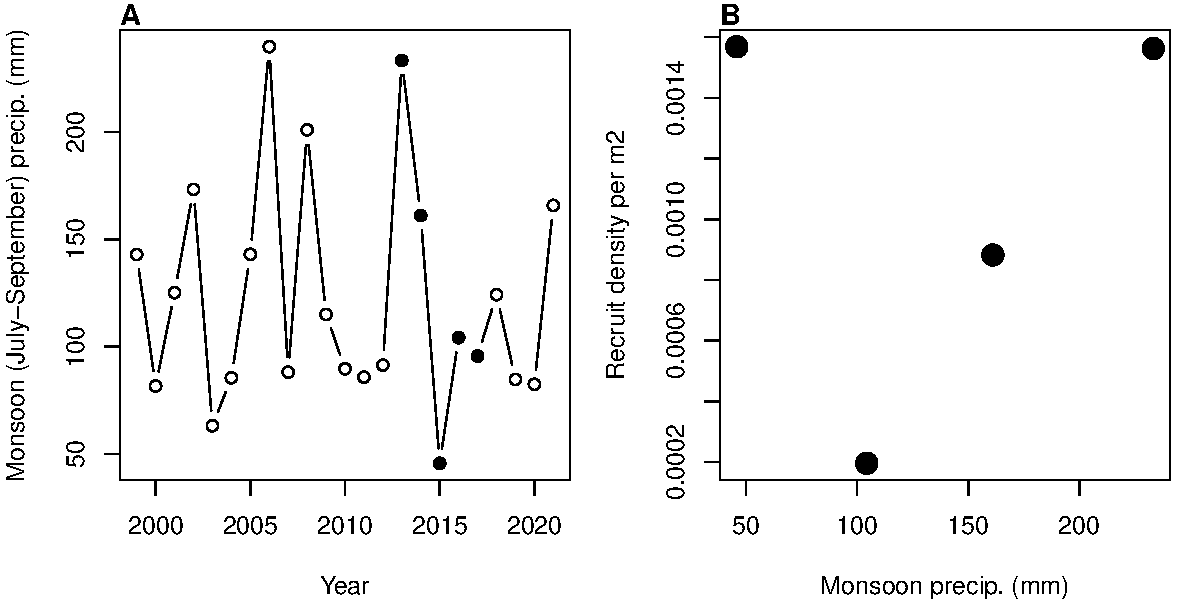
\includegraphics[width=\linewidth]{Figures/monsoon_seedlings}
  \caption{A, Time series of annual monsoon precipitation (filled circles are the years in which this study was conducted). B, Relationship between density of creosotebush recruits observed on our transects in May-June and monsoon precipitation in the preceding July-September.}
  \label{fig:monsoon}
  \end{center}
\end{figure}

\end{document}
